%%%%%%%%%%%%%%%%%%%%%%%%%%%%%%%%%%%%%%%%%
% Ariadne Assignment
%
% This template originates from:
% http://www.LaTeXTemplates.com
%
% Authors:
% Marion Lachaise & François Févotte
% Vel (vel@LaTeXTemplates.com)
%
% License:
% CC BY-NC-SA 3.0 (http://creativecommons.org/licenses/by-nc-sa/3.0/)
% 
%%%%%%%%%%%%%%%%%%%%%%%%%%%%%%%%%%%%%%%%%

%----------------------------------------------------------------------------------------
%	PACKAGES AND OTHER DOCUMENT CONFIGURATIONS
%----------------------------------------------------------------------------------------

\documentclass{article}

\usepackage{hyperref}
\usepackage{graphicx} 
\usepackage{float}
\usepackage[autoplay,loop]{animate}

%%%%%%%%%%%%%%%%%%%%%%%%%%%%%%%%%%%%%%%%%
% Lachaise Assignment
% Structure Specification File
% Version 1.0 (26/6/2018)
%
% This template originates from:
% http://www.LaTeXTemplates.com
%
% Authors:
% Marion Lachaise & François Févotte
% Vel (vel@LaTeXTemplates.com)
%
% License:
% CC BY-NC-SA 3.0 (http://creativecommons.org/licenses/by-nc-sa/3.0/)
% 
%%%%%%%%%%%%%%%%%%%%%%%%%%%%%%%%%%%%%%%%%

%----------------------------------------------------------------------------------------
%	PACKAGES AND OTHER DOCUMENT CONFIGURATIONS
%----------------------------------------------------------------------------------------

\usepackage{amsmath,amsfonts,stmaryrd,amssymb} % Math packages

\usepackage{enumerate} % Custom item numbers for enumerations

\usepackage[ruled]{algorithm2e} % Algorithms

\usepackage[framemethod=tikz]{mdframed} % Allows defining custom boxed/framed environments

\usepackage{listings} % File listings, with syntax highlighting
\lstset{
	basicstyle=\ttfamily, % Typeset listings in monospace font
}

%----------------------------------------------------------------------------------------
%	DOCUMENT MARGINS
%----------------------------------------------------------------------------------------

\usepackage{geometry} % Required for adjusting page dimensions and margins

\geometry{
	paper=a4paper, % Paper size, change to letterpaper for US letter size
	top=2.5cm, % Top margin
	bottom=3cm, % Bottom margin
	left=2.5cm, % Left margin
	right=2.5cm, % Right margin
	headheight=14pt, % Header height
	footskip=1.5cm, % Space from the bottom margin to the baseline of the footer
	headsep=1.2cm, % Space from the top margin to the baseline of the header
	%showframe, % Uncomment to show how the type block is set on the page
}

%----------------------------------------------------------------------------------------
%	FONTS
%----------------------------------------------------------------------------------------

\usepackage[utf8]{inputenc} % Required for inputting international characters
\usepackage[T1]{fontenc} % Output font encoding for international characters

\usepackage{XCharter} % Use the XCharter fonts

%----------------------------------------------------------------------------------------
%	COMMAND LINE ENVIRONMENT
%----------------------------------------------------------------------------------------

% Usage:
% \begin{commandline}
%	\begin{verbatim}
%		$ ls
%		
%		Applications	Desktop	...
%	\end{verbatim}
% \end{commandline}

\mdfdefinestyle{commandline}{
	leftmargin=10pt,
	rightmargin=10pt,
	innerleftmargin=15pt,
	middlelinecolor=black!50!white,
	middlelinewidth=2pt,
	frametitlerule=false,
	backgroundcolor=black!5!white,
	frametitle={Command Line},
	frametitlefont={\normalfont\sffamily\color{white}\hspace{-1em}},
	frametitlebackgroundcolor=black!50!white,
	nobreak,
}

% Define a custom environment for command-line snapshots
\newenvironment{commandline}{
	\medskip
	\begin{mdframed}[style=commandline]
}{
	\end{mdframed}
	\medskip
}

%----------------------------------------------------------------------------------------
%	FILE CONTENTS ENVIRONMENT
%----------------------------------------------------------------------------------------

% Usage:
% \begin{file}[optional filename, defaults to "File"]
%	File contents, for example, with a listings environment
% \end{file}

\mdfdefinestyle{file}{
	innertopmargin=1.6\baselineskip,
	innerbottommargin=0.8\baselineskip,
	topline=false, bottomline=false,
	leftline=false, rightline=false,
	leftmargin=2cm,
	rightmargin=2cm,
	singleextra={%
		\draw[fill=black!10!white](P)++(0,-1.2em)rectangle(P-|O);
		\node[anchor=north west]
		at(P-|O){\ttfamily\mdfilename};
		%
		\def\l{3em}
		\draw(O-|P)++(-\l,0)--++(\l,\l)--(P)--(P-|O)--(O)--cycle;
		\draw(O-|P)++(-\l,0)--++(0,\l)--++(\l,0);
	},
	nobreak,
}

% Define a custom environment for file contents
\newenvironment{file}[1][File]{ % Set the default filename to "File"
	\medskip
	\newcommand{\mdfilename}{#1}
	\begin{mdframed}[style=file]
}{
	\end{mdframed}
	\medskip
}

%----------------------------------------------------------------------------------------
%	NUMBERED QUESTIONS ENVIRONMENT
%----------------------------------------------------------------------------------------

% Usage:
% \begin{question}[optional title]
%	Question contents
% \end{question}

\mdfdefinestyle{question}{
	innertopmargin=1.2\baselineskip,
	innerbottommargin=0.8\baselineskip,
	roundcorner=5pt,
	nobreak,
	singleextra={%
		\draw(P-|O)node[xshift=1em,anchor=west,fill=white,draw,rounded corners=5pt]{%
		Question \theQuestion\questionTitle};
	},
}

\newcounter{Question} % Stores the current question number that gets iterated with each new question

% Define a custom environment for numbered questions
\newenvironment{question}[1][\unskip]{
	\bigskip
	\stepcounter{Question}
	\newcommand{\questionTitle}{~#1}
	\begin{mdframed}[style=question]
}{
	\end{mdframed}
	\medskip
}

%----------------------------------------------------------------------------------------
%	WARNING TEXT ENVIRONMENT
%----------------------------------------------------------------------------------------

% Usage:
% \begin{warn}[optional title, defaults to "Warning:"]
%	Contents
% \end{warn}

\mdfdefinestyle{warning}{
	topline=false, bottomline=false,
	leftline=false, rightline=false,
	nobreak,
	singleextra={%
		\draw(P-|O)++(-0.5em,0)node(tmp1){};
		\draw(P-|O)++(0.5em,0)node(tmp2){};
		\fill[black,rotate around={45:(P-|O)}](tmp1)rectangle(tmp2);
		\node at(P-|O){\color{white}\scriptsize\bf !};
		\draw[very thick](P-|O)++(0,-1em)--(O);%--(O-|P);
	}
}

% Define a custom environment for warning text
\newenvironment{warn}[1][Warning:]{ % Set the default warning to "Warning:"
	\medskip
	\begin{mdframed}[style=warning]
		\noindent{\textbf{#1}}
}{
	\end{mdframed}
}

%----------------------------------------------------------------------------------------
%	INFORMATION ENVIRONMENT
%----------------------------------------------------------------------------------------

% Usage:
% \begin{info}[optional title, defaults to "Info:"]
% 	contents
% 	\end{info}

\mdfdefinestyle{info}{%
	topline=false, bottomline=false,
	leftline=false, rightline=false,
	nobreak,
	singleextra={%
		\fill[black](P-|O)circle[radius=0.4em];
		\node at(P-|O){\color{white}\scriptsize\bf i};
		\draw[very thick](P-|O)++(0,-0.8em)--(O);%--(O-|P);
	}
}

% Define a custom environment for information
\newenvironment{info}[1][Info:]{ % Set the default title to "Info:"
	\medskip
	\begin{mdframed}[style=info]
		\noindent{\textbf{#1}}
}{
	\end{mdframed}
}
 % Include the file specifying the document structure and custom commands

%----------------------------------------------------------------------------------------
%	ASSIGNMENT INFORMATION
%----------------------------------------------------------------------------------------

\title{ARIADNE: supporto e integrazione di GNUPLOT} % Title of the assignment

\author{Albanese Mirko\\ \texttt{mirko.albanese@studenti.univr.it}} % Author name and email address

\date{Univeristà degli studi di Verona --- \today} % University, school and/or department name(s) and a date

%----------------------------------------------------------------------------------------

\begin{document}

\maketitle % Print the title

%----------------------------------------------------------------------------------------
%	INTRODUCTION
%----------------------------------------------------------------------------------------

\section*{Introduzione} % Unnumbered section
In Ariadne vi è la necessità di implementare un'interfaccia che permetta di disegnare la regione raggiunta di un sistema a derivate parziali. Al suo interno vi è già l'utility Cairo che mediante il plotting png permette di disegnare la traiettoria nel tempo di un sistema ad equazioni differenziali ordinarie. Questo documento descrive l'attività svolta per implementare un supporto a Gnuplot, con lo scopo di poter disegnare sistemi a derivate parziali, ovvero la loro regione raggiunta.

Nella prima sezione viene descritto il funzionamento di Gnuplot come la sua installazione e il suo funzionamento.

Nella seconda sezione vengono illustrati gli obiettivi posti e le motivazioni che hanno spinto a costruire il supporto e viene descritto brevemente i modelli utilizzati per testare il supporto, in particolare \verb|l'equazione dell'onda|.

Nella terza sezione viene descritto l'interfacciamento a Gnuplot all'interno dell'interfaccia di disegno preesistente in Ariadne.

Nella quarta sezione viene illustrato il risultato finale ottenuto, mostrando il file generato dall'interfaccia di disegno Gnuplot.



\section{Gnuplot}

Gnuplot è un'utilità grafica portable basata su riga di comando per Linux, OS/2, MS Windows, OSX, VMS e molte altre piattaforme. Il codice sorgente è protetto da copyright ma distribuito liberamente. È stato originariamente creato per consentire a scienziati e studenti di visualizzare funzioni e dati matematici in modo interattivo, ma è cresciuto fino a supportare molti usi non interattivi come lo scripting web. Viene anche utilizzato come motore di stampa da applicazioni di terze parti come Octave. 
Gnuplot supporta molte tipologie di grafici in 2D e 3D. Può disegnare usando linee, punti, riquadri, contorni,
campi vettoriali, superfici e vari testi associati.

%------------------------------------------------

\subsection{Installazione}
Per evitare incongruenze con la libreria Ariadne si preferisce installare programmi e utility da pacchetti, perciò si consiglia fortemente di installare la versione che in questo momento, da pacchetto apt è la versione 5.2.8 oppure indirizzarsi al sito internet \url{http://sourceforge.net/projects/gnuplot} e scaricare la versione 5.2.8.\newline
Per installare la versione da apt occorre digitare il seguente comando da shell:
\begin{commandline}
	\begin{verbatim}
		$sudo apt-get install gnuplot
	\end{verbatim}
\end{commandline}

Altrimenti una volta scaricato, estratto il sorgente e portatosi all'interno della cartella di installazione, l'installazione avviene digitando i seguenti comandi:\newline
\begin{commandline}
\begin{verbatim}
$./configure
$make
$make check
$make install
\end{verbatim}
\end{commandline}
Per verificare la corretta installazione basti digitare sulla shell il comando 
\begin{verbatim}
gnuplot
\end{verbatim}
per poter avviare l'applicazione.\newline

Un ulteriore controllo da effettuare è verificare se gnuplot ha installato tutte le tipologie di output che ci interessano, per fare questo, avviate l'applicazione inserendo il comando 
\begin{verbatim}
gnuplot
\end{verbatim}
succettivamente per visualizzare le tipologie di output installate occore eseguire il comando:
\begin{verbatim}
set terminal
\end{verbatim}
e tra l'elenco su schermo devono apparire la dicitura gif e png. Se ciò non dovesse accadere allora occorre installare la libreria libgd-dev mediante il comando:
\begin{verbatim}
sudo apt-get install libgd-dev
\end{verbatim}
e una volta installato ripetere il procedimento di installazione di gnuplot descritto sopra.

%------------------------------------------------

\subsection{Funzionamento}
Come si è potuto facimente notare l'utilizzo di gnuplot è basato sull'esecuzione, da riga di comando, di una serie consecutiva di comandi che, fino alla costruzione del disegno finale, permettono di creare il disegno da una fonti di dati in input come un file oppure una serie di valori.
Ora verranno descritti brevemente i comandi che interessano maggiormente per la comprensione del progetto.\newline

Gnuplot permette di creare un canvas di un determinato tipo (png, gif etc) di date dimensioni mediante il comando:
\begin{verbatim}
set terminal [type] size [xvalue], [yvalue]
\end{verbatim}
dove [type] può essere un elemento tra quelli definiti digitando 'set terminal' dopo aver avviato gnuplot e [xvalue] e [yvalue] sono rispettivamente le dimensioni dell'immagine.\newline

Successivamente gnuplot ci permette di definire il nome del file di output mediante il comando:
\begin{verbatim}
set output "NOME_FILE.xxx"
\end{verbatim}

Permette di disegnare un elemento sopra un altro oppure rendere il plot univoco all'elemento disegnato mediante il comando:
\begin{verbatim}
set multiplot or unset multiplot
\end{verbatim}

Permette, inoltre di definire un nome e un range agli assi cartesiani mediante i comandi:
\begin{verbatim}
set xlabel 'x0'
set ylabel 'x1'
set zlabel 'x2'
set xrange [0:19] 
set yrange [0:19] 
set zrange [0:1] 
\end{verbatim}

Permette di definire una color palette (utilizzato nelle proiezioni 3d) mediante i seguenti comandi:
\begin{verbatim}
set cbrange [-0.5:1]
set cbtics 0.2
set palette defined
\end{verbatim}

Permette di definire una trasparenza:
\begin{verbatim}
set style fill transparent solid #
\end{verbatim}

Infine permette di disegnare a 2 dimensioni:
\begin{verbatim}
plot '-' 
\end{verbatim}

Oppure a 3 dimensioni:
\begin{verbatim}
splot '-'
\end{verbatim}

Il digit '-' permette a gnuplot di sapere che dopo il seguente comando vi saranno degli input che verranno inseriti (ogni input deve essere confermato con il ritorno a capo) e terminati con la lettera 'e'.
\newline

Infine per terminare il suo utilizzo viene digitato il comando:
\begin{verbatim}
quit
\end{verbatim}

%------------------------------------------------
\section{Obiettivi}

%------------------------------------------------

\subsection{Motivazioni}

Durante lo sviluppo del progetto si è posto il problema di poter visualizzare graficamente la regione raggiunta di un sistema a derivate parziali. Questa necessità ha permesso di progettare un supporto a Gnuplot all'interno di Ariadne per gestire, oltre alla stampa di un disegno statico, un'animazione e di conseguenza visualizzare la regione raggiunta nel tempo sulle coordinate spaziali, ma anche una visualizzazione statica, sia di una proiezione di una variabile spaziale che una traiettoria nel tempo.
Per fare ciò, ho costruito una simulazione a due dimensioni (x1, t) e a tre dimensioni (x1, x2, t) dell'equazione dell'onda per poter testare il comportamento di Gnuplot.

\subsection{Equazione dell'onda}
In questa sotto-sezione viene descritta brevemente l'implementazione utilizzata per simulare l'equazione dell'onda a due e a tre dimensioni. In entrambe le metodologie viene utilizzato l'algoritmo delle differenze finite per risolvere numericamente le equazioni differenziali.

\subsubsection{Due dimensioni: Spazio x1 - Tempo t}
L'equazione dell'onda a 2 dimensioni può essere paragonata al movimento di una corda vibrante.
L'equazione che modella questa situazione può essere scritta nel seguente modo (equazione dell'onda):

\begin{equation}
	\frac{\partial^2u}{\partial t^2} = c^2\frac{\partial^2u}{\partial x^2}
\end{equation}

dove, $u(x, t)$ è lo spostamento della corda.

Definiamo ora gli elementi principali per definire la simulazione:

\begin{itemize}
\item Definire un quadro dimensionale dell'equazione 1, ovvero: $x \in (0,L), t \in (0, T] $
\item Definire una condizione iniziale sulla posizione: $u(x, 0) = I(x) $
\item Definire una condizione iniziale sulla velocità: $\frac{\partial}{\partial t}u(x, 0) = 0 $
\item Definire una condizione iniziale al contorno: $x(0, t) = x(L, t) = 0 $
\end{itemize}

Una volta definite le condizioni iniziali occorre discretizzare le variabili di spazio e di tempo definendo una mesh per variabile dove ogni punto è equidistante da quello successivo rendendo la mesh spaziale e temporale uniformi.

\begin{itemize}
\item[Tempo] : $0=t_0<t_1<t_2<...<t_{N_{t-1}}<t_{N_t}=T$
\item[Spazio] : $0=x_0<x_1<x_2<...<x_{N_{x-1}}<x_{N_x}=L$
\end{itemize}

Ogni elemento $x_i$ e $t_i$ ha una spaziatura $\delta x$ e $\delta t$ uniforme:

\begin{itemize}
\item[Tempo] : $t_i=i\Delta t. i=0...N_t$
\item[Spazio] : $t_i=i\Delta x. i=0...N_x$
\end{itemize}

La soluzione all'interno della mesh viene così definita $u{_x}{^n}=u(x_i,t_n)$.

Sostituendo la soluzione all'interno dell'equazione 1 otteniamo la seguente equazione differenziale.

\begin{equation}
	\frac{\partial^2}{\partial t^2}u(x_i,t_n) = c^2\frac{\partial^2}{\partial x ^2}u(x_i,t_n)
\end{equation}

dove, $i = 1,...,N_x-1$ e $n = 1,...,N_t-1$.
Per $n=0$ avremo la condizione iniziale $u = I(x)$ mentre per $i={0,N_x}$ avremo le condizioni al contorno con $u = 0$.

Applicando il metodo delle differenze finite all'equazione 2 possiamo ottenere:

\begin{equation}
\frac{\partial^2}{\partial t^2}u(x_i,t_n) \simeq \frac{u^{n+1}_x-2u{^n}_x+u^{n-1}_x}{\Delta t^2}
\end{equation}

e

\begin{equation}
\frac{\partial^2}{\partial x^2}u(x_i,t_n) \simeq \frac{u^n_{x+1}-2u{^n}_x+u^{n}_{x+1}}{\Delta x^2}
\end{equation}

ottenendo la sequente equazione

\begin{equation}
\frac{u^{n+1}_x-2u{^n}_x+u^{n-1}_x}{\Delta t^2} = c^2\frac{u^n_{x+1}-2u{^n}_x+u^{n}_{x+1}}{\Delta x^2}
\end{equation}

Da qui si deve definire la versione algebrica della condizione iniziale $u_t(x,0)=0$ definendo $u_x{^0}=I(x_i)$ con $u{_x}^{n-1} = u_x^{n+1}$ per $n=0$

Risolvendo per $u{_x}^{n+1}$ dall'equazione 5 possiamo scrivere la sequente equazione:

\begin{equation}
u{_x}^{n+1} = -u{_x}^{n-1}+2u{_x}^n+C^2(u_{x+1}^n-2u{_x}^n+u_{x-1}^n)
\end{equation}

Avendo 3 step $u_{x}^{n-1}$, $u_{x}^{n}$, $u_{x}^{n+1}$, occorre definire la soluzione all'istante temporale $n=0$ perchè in questa situazione $u_{x}^{n-1}$ punterà ad un valore al di fuori dalla mesh. Perciò considerando $u_{x}^{n-1} = u_{x}^{n+1}$ possiamo definire

\begin{equation}
u_{x}^1 = u_{x}^0 + \frac{1}{2}C^2(u_{i+1}^n - 2u_{i}^n + u_{i-1}^n
\end{equation}

dove $C=c \frac{\Delta t}{\Delta x}$ viene denominato Courant Number. 
In questo modo è possibile trovare la soluzione all'istante di tempo successivo.

L'algoritmo è il seguente:

\begin{center}
	\begin{minipage}{0.5\linewidth} % Adjust the minipage width to accomodate for the length of algorithm lines
		\begin{algorithm}[H]
			\KwIn{$I(x)$, Condizione iniziale}  % Algorithm inputs
			\KwIn{$u[i]$, Vettore dei $u{_x}^{n+1}$}
			\KwIn{$u_1[i]$, Vettore dei $u{_x}^{n}$}
			\KwIn{$u_2[i]$, Vettore dei $u{_x}^{n-1}$}
			\KwResult{$(u)$, Soluzione} % Algorithm outputs/results
			\medskip
			Risolvere $u{_x}^0=I(x), \forall x$\;
			Risolvere $u{_x}^1$\;
			Forzare le condizioni al contorno \;
			$\forall n \rightarrow u{_x}^{n+1}$ \;
			\caption{\texttt{2D Wave equation solver}} % Algorithm name
			\label{alg:2D Wave equation solver}   % optional label to refer to
		\end{algorithm}
	\end{minipage}
\end{center}


\subsubsection{Tre dimensioni: Spazio x1 - Spazio x2 - Tempo t}
L'equazione dell'onda a 3 dimensioni può essere paragonata al movimento di un telo elastico. L'equazione che modella questa situazione può essere scritta nel seguente modo, in maniera molto simile a quella a due dimensioni (equazione dell'onda):

\begin{equation}
	\frac{\partial^2u}{\partial t^2} = c^2(\frac{\partial^2u}{\partial x^2} + \frac{\partial^2u}{\partial y^2})
\end{equation}

La discretizzazione dell'equazione avviene allo stesso modo del paragrafo in riferimento all'equazione dell'onda a 2 dimensioni, in particolare:

\begin{equation}
\frac{u_{x,y}^{n+1}-2u_{x,y}^n+u_{x,y}^{n-1}}{\Delta t^2}=C^2\frac{u_{x+1,y}^n-2u_{x,y}^n+u_{x-1,y}^n}{\Delta x^2}+c^2\frac{u_{x,y+1}^n-2u_{x,y}^n+u_{x,y-1}^n}{\Delta y^2}
\end{equation}

Risolvendo per $u_{x,y}^{n+1}$ avremo

\begin{equation}
u_{x,y}^{n+1} = 2u_{x,y}^n+u_{i,j}^{n-1}+c^2\Delta t^2(\frac{u_{x+1,y}^n-2u_{x,y}^n+u_{x-1,y}^n}{\Delta x^2}+\frac{u_{x,y+1}^n-2u_{x,y}^n+u_{x,y-1}^n}{\Delta y^2})
\end{equation}

Come nel caso a 2 dimensioni vi è lo stesso problemo all'instante temporale $n=0$ in cui $u_{i,j}^{n-1}$ punta ad un valore al di fuori dalla mesh. La stessa situazione viene applicata in questo contesto.

\begin{equation}
u_{x,y}^{n+1} = u_{x,y}^n + \frac{1}{2}c^2\Delta t^2(\frac{u_{x+1,y}^n-2u_{x,y}^n+u_{x-1,y}^n}{\Delta x^2}+\frac{u_{x,y+1}^n-2u_{x,y}^n+u_{x,y-1}^n}{\Delta y^2})
\end{equation}

L'algoritmo è il seguente

\begin{center}
	\begin{minipage}{0.5\linewidth} % Adjust the minipage width to accomodate for the length of algorithm lines
		\begin{algorithm}[H]
			\KwIn{$I(x,y)$, Condizione iniziale}  % Algorithm inputs
			\KwIn{$u[i]$, Vettore dei $u{_x}^{n+1}$}
			\KwIn{$u_1[i]$, Vettore dei $u{_x}^{n}$}
			\KwIn{$u_2[i]$, Vettore dei $u{_x}^{n-1}$}
			\KwResult{$(u)$, Soluzione} % Algorithm outputs/results
			\medskip
			Risolvere $u_{x,y}^0=I(x,y), \forall x,y$\;
			Risolvere $u_{x,y}^1$\;
			Forzare le condizioni al contorno $x$ e $y$\;
			$\forall n \rightarrow u_{x,y}^{n+1}$ \;
			\caption{\texttt{3D Wave equation solver}} % Algorithm name
			\label{alg:3D Wave equation solver}   % optional label to refer to
		\end{algorithm}
	\end{minipage}
\end{center}

%----------------------------------------------------------------------------------------
%	PROBLEM 2
%----------------------------------------------------------------------------------------
\section{Implementazione}
In questa sezione viene descritto il lavoro svolto per integrare al meglio il supporto di Gnuplot all'interno dell'interfaccia di disegno di Ariadne.

\subsection{Gnuplot-iostream}
Gnuplot permette il suo funzionamento mediante l'invocazione consecutiva di comandi, il tutto mediante un'interazione da shell. Perciò serve un intermediario tra il framework Ariadne (C++) e l'invocazione dei comandi verso l'istanza Gnuplot. Per fare ciò Daniel Stahlke (dan@stahlke.org) ha sviluppato un'interfaccia C++ verso Gnuplot, chiamata gnuplot-iostream. Questa interfaccia permette, tramite pipe, di propagare i comandi gnuplot verso lo standard output mediante l'utilizzo di File. L'interfaccia di Daniel però presentava un enorme problema per la filosofia di Ariadne, ovvero utilizza le librerie Boost per gestire i descrittori dei file e di conseguenza il buffering verso lo standard output. Alcune librerie esterne presentano un problema di compatibilità nel tempo, perciò si è deciso di eliminare Boost dall'interfaccia. L'utilizzo della libreria Boost all'interno di gnuplot-iostream veniva utilizzata solamente per definire il descrittore del file e per poterlo utilizzare verso lo standard output mediante pipe, perciò ho creato la funzionalità che sostituisce il relativo funzionamento utilizzando le classi \verb|std::streambuf| e \verb|std::ostream|.

\subsection{Interfacciamento verso la libreria Ariadne}
Dopo aver integrato l'interfaccia C++ - Gnuplot all'interno di Ariadne, era fondamentale capire come doveva essere gestito l'utilizzo di Gnuplot. L'interfaccia di disegno in Ariadne permette di disegnare all'interno di un canvas una serie di coordinate appartenenti ad una figura, in cui vi si può associare determinate proprietà come ad esempio il colore e lo spessore della linea, il riempimento, l'opacità e così via. 
I metodi di disegno sono inseriti in una classe virtuale chiamata \verb|CanvasInterface| permettendo a diverse "utility" di interfacciarsi e appoggiarsi a questi metodi per poter disegnare una determinata figura. Ad oggi Ariadne utilizza Cairo come utility predefinita di un disegno statico e Gnuplot come utility aggiuntiva per disegnare sia disegni statici che disegni dinamici.

Questi aspetti sono stati fondamentali da capire perchè Gnuplot doveva utilizzare l'interfaccia preesistente e di conseguenza l'implementazione doveva essere il più generica possibile. Dal versante Gnuplot, invece, è stato fondamentale capire ogni suo punto debole e ogni suo punto di forza, andando ad analizzare ogni sua modalità di utilizzo.

Queste analisi mi hanno portato a creare una classe adibita all'utilizzo di Gnuplot chiamata \verb|GnuplotCanvas| dove al suo interno sono stati definiti tutti i metodi provenienti da \verb|CanvasInterface| per la creazione del disegno e inoltre i metodi proprietari di gnuplot per l'invocazione dei comandi utilizzati per definire ogni proprietà del disegno.

\subsection{Estensione della classe DrawableInterface e integrazione di Tensor}
Gnuplot può permettere una stampa 3D fornendo comandi adatti alla stampa a tre dimensioni, perciò vi è stata la necessità di integrare la classe \verb|DrawableInterface| in modo che determinati oggetti possano essere identificati e disegnati come oggetti a due dimensioni oppure a tre dimensioni, dove questi ultimi possono essere proiezioni a due dimensioni. La classe \verb|DrawableInterface| viene sostituita con due classi: \verb|Drawable2dInterface| che definisce e disegna gli oggetti a 2 dimensioni, la classe \verb|Drawabe2d3dInterface| che estende \verb|Drawable2dInterface| definendo e disegnando gli oggetti a 3 dimensioni ma che permettono anche proiezioni a 2 dimensioni.

Viene quindi integrata e modificata la classe \verb|Tensor| estendedola con la classe \verb|Drawabe2d3dInterface| per poter definire così l'oggetto Tensore che può assumere forme a tre dimensioni ma anche proiezioni su due dimensioni.

\subsection{Estensione della classe Figure}
Dopo aver aggiunto la modalità di disegno in 3 dimensione, è necessario estendere la classe 3D inserendo i vari metodi relativi alla gestione di una figura a tre dimensioni e aggiungendo e estendendo la chiamata al costruttore dell'utility Gnuplot in aggiunta alla già esistente chiamata al costruttore per l'utility Cairo.

\subsection{Creazione del file di dump}
Ad ogni stampa di un disegno, l'interfaccia genera automaticamente un file con estensione \verb|.gnu| con al suo interno la lista dei comandi Gnuplot che l'interfaccia ha eseguito e che ha passato alla pipe in standard output. Questo file può essere utilizzato come metodo di debug per verificare il corretto funzionamento oppure può essere importato da un software che utilizza un engine Gnuplot per poter visualizzare il disegno da un tool esterno.

\section{TEST}
Una volta conclusa l'implementazione e l'integrazione ho utilizzato le simulazioni dell'equazione dell'onda create per costruire dei semplici casi di test per poter testare l'interfacciamento a Gnuplot. I seguenti test sono presenti all'interno del file \verb|test_gnuplot.cpp|, eccone i relativi risultati:

\subsubsection{Generazione di un punto}
\begin{figure}[H] 
\begin{center}  
  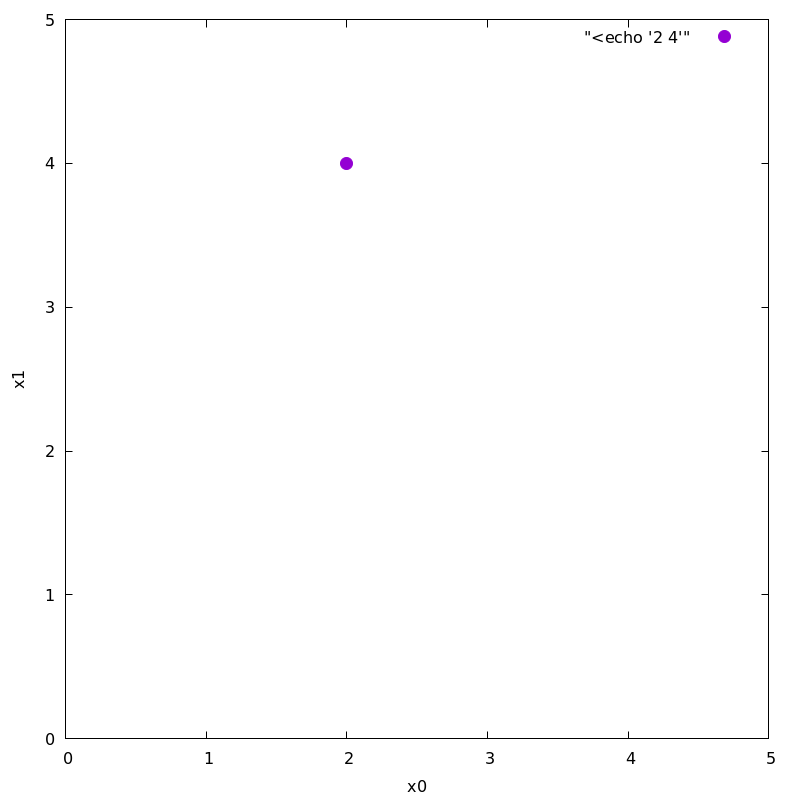
\includegraphics[width=10cm]{test-gnuplot-point2d.png}\\ 
  \caption{Stampa di un punto nello spazio bidimensionale} 
\end{center} 
\end{figure}

\subsubsection{Generazione di una linea}

\begin{figure}[H] 
\begin{center}  
  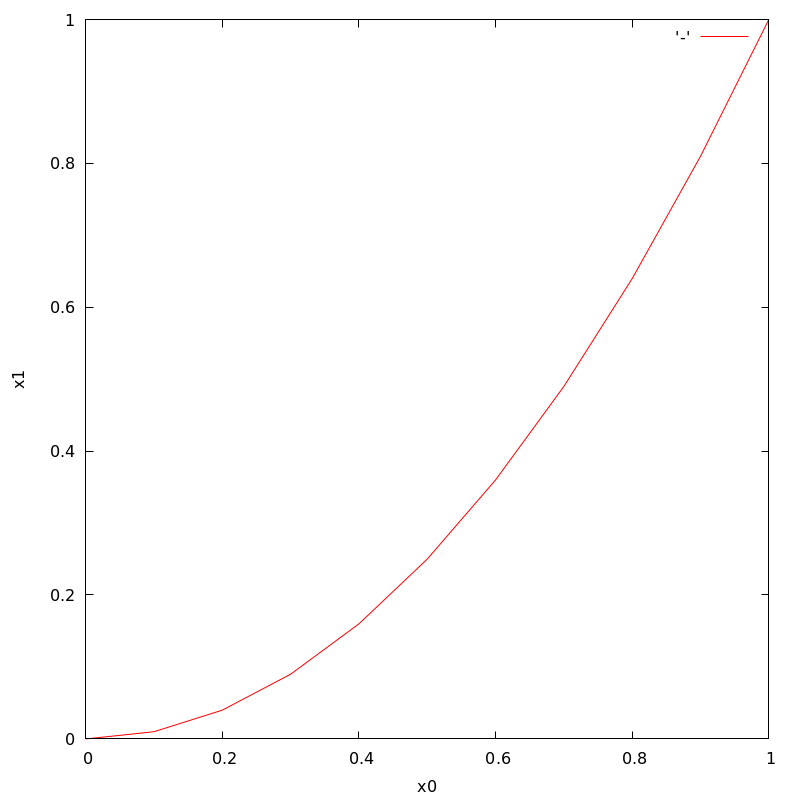
\includegraphics[width=10cm]{test_gnuplot-curve.png}\\ 
  \caption{Stampa di una linea nello spazio bidimensionale} 
\end{center} 
\end{figure}

\subsubsection{Animazione di una corda vibrante secondo l'equazione dell'onda}

\begin{frame}{Animazione di una corda vibrante}
\animategraphics[controls,width=10cm]{5}{string/animate_}{0}{36}
\end{frame}

\subsubsection{Generazione di una gaussiana a tre dimensioni}

\begin{figure}[H] 
\begin{center}  
  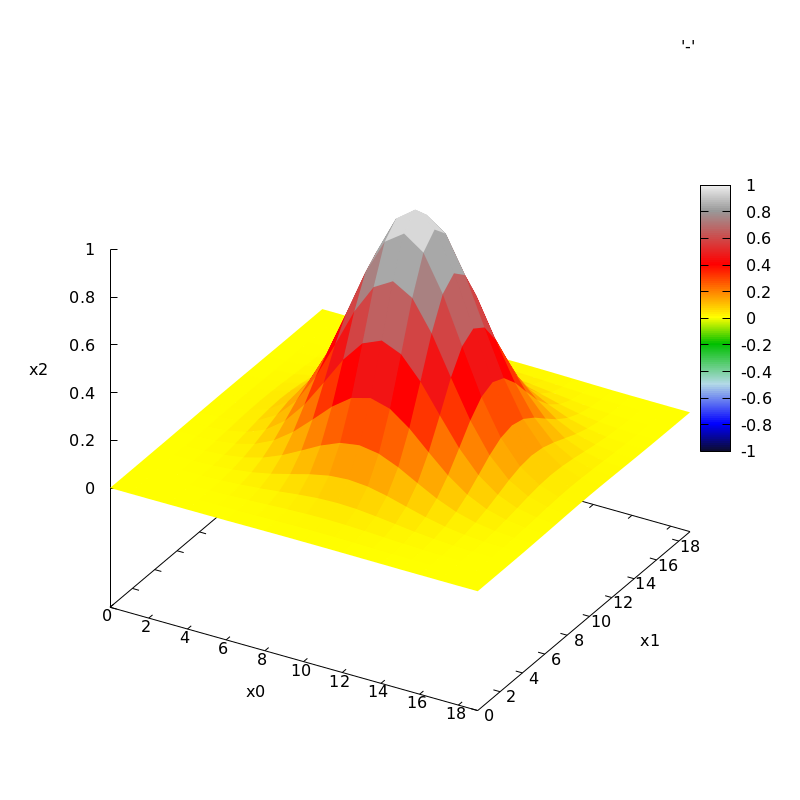
\includegraphics[width=10cm]{test-gnuplot-Gauss3D.png}\\ 
  \caption{Stampa di una gaussiana nello spazio tridimensionale} 
\end{center} 
\end{figure}

\subsubsection{Proiezione X0X1 di una gaussiana a tre dimensioni}

\begin{figure}[H] 
\begin{center}  
  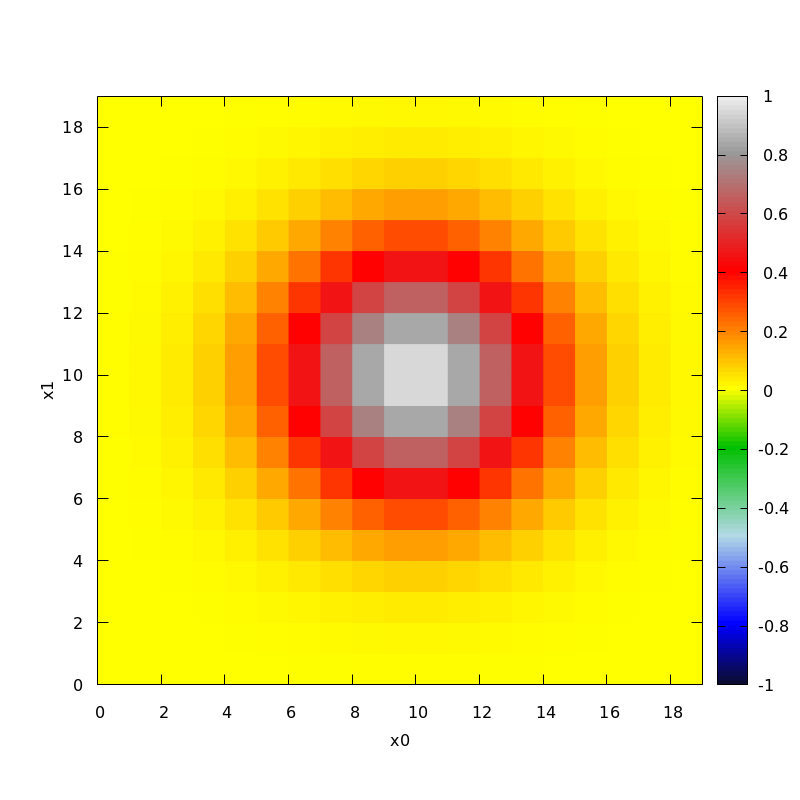
\includegraphics[width=9cm]{test-gnuplot-Gauss3DProjXY.png}\\ 
  \caption{Stampa di una proiezione delle dimensioni x0 e x1 di una gaussiana nello spazio tridimensionale} 
\end{center} 
\end{figure}

\subsubsection{Proiezione X0X2 di una gaussiana a tre dimensioni}

\begin{figure}[H] 
\begin{center}  
  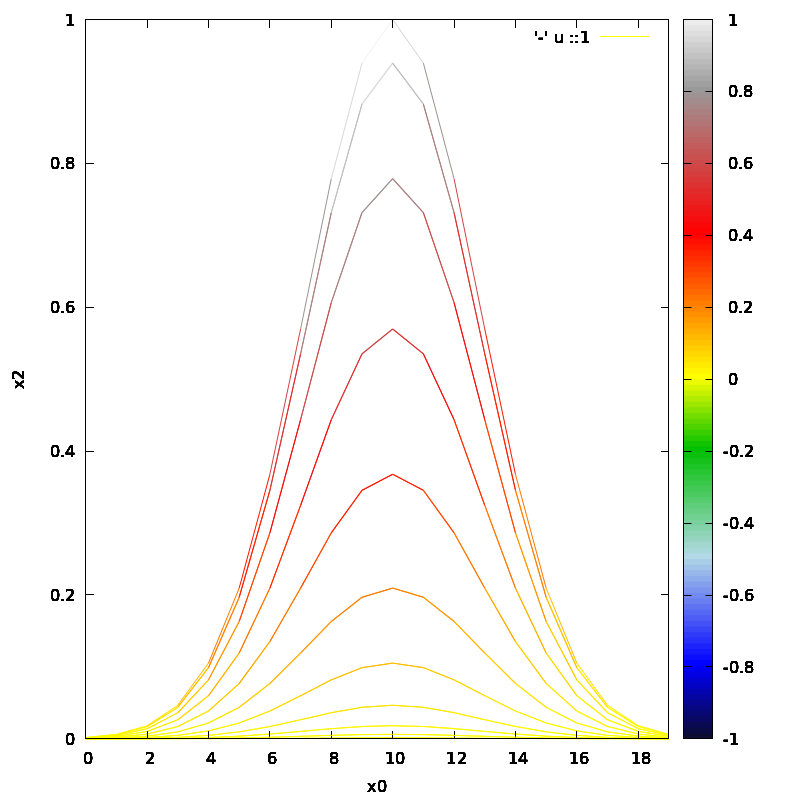
\includegraphics[width=9cm]{test-gnuplot-Gauss3DProjXZ.png}\\ 
  \caption{Stampa di una proiezione delle dimensioni x0 e x2 di una gaussiana nello spazio tridimensionale} 
\end{center} 
\end{figure}

\subsubsection{Proiezione X1X2 di una gaussiana a tre dimensioni}

\begin{figure}[H] 
\begin{center}  
  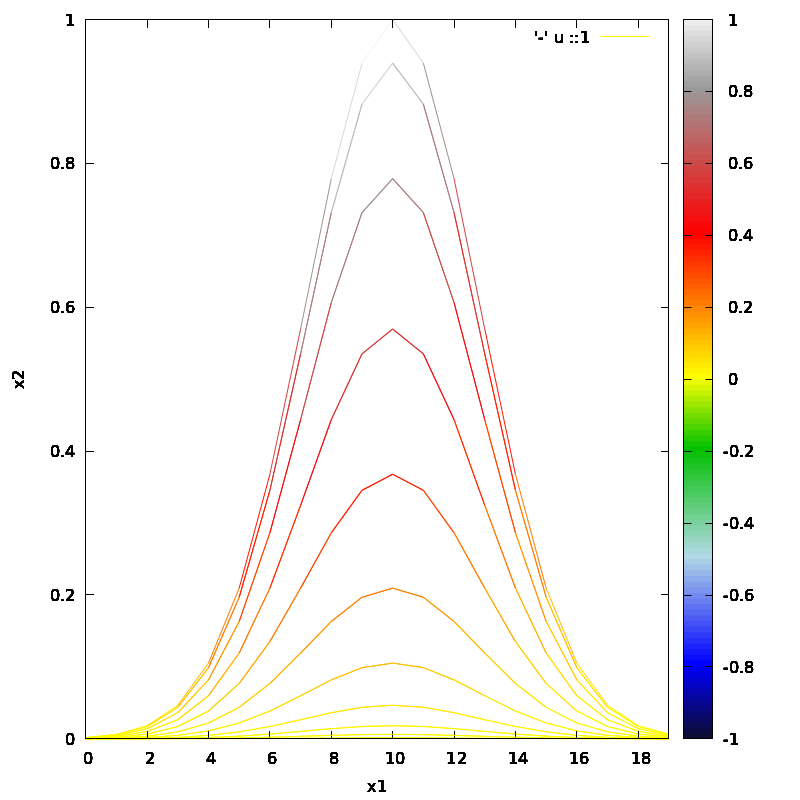
\includegraphics[width=10cm]{test-gnuplot-Gauss3DProjYZ.png}\\ 
  \caption{Stampa di una proiezione delle dimensioni x1 e x2 di una gaussiana nello spazio tridimensionale} 
\end{center} 
\end{figure}

\subsubsection{Animazione di una gaussiana a tre dimensioni secondo l'equazione dell'onda}

\begin{frame}{Animazione di una gaussiana}
\animategraphics[controls,width=10cm]{5}{gauss/animate_}{0}{21}
\end{frame}

\section{CONCLUSIONE E SVILUPPI FUTURI}
In conclusione questo lavoro permette di avere una base, all'interno del framework C++ Ariadne per poter visualizzare la regione raggiunta di un sistema a derivate parziali andando a rappresentare sia nel tempo con disegni dinamici (animazioni) che nello spazio mediante disegni statici. Inoltre permette di poter definire una modalità di stampa definita da Gnuplot, oltre alla già esistente Cairo.

In merito ai sviluppi futuri sicuramente sarà presente il mantenimento dell'interfaccia e l'espansione della stessa in base alle esigenze dettate da Ariadne.

\end{document}
